\documentclass[11pt,a4paper]{article}
\usepackage[utf8x]{inputenc}
\usepackage[T1]{fontenc}
\usepackage{color}
\usepackage{multicol}
\usepackage{array}%création tableaux
\usepackage{graphicx}%pour les photosimages
%\usepackage{gentium}

\usepackage{fancyhdr}
%\pagestyle{fancy}
%\renewcommand{\headrulewidth}{0pt}
%\renewcommand{\footrulewidth}{0pt}
%\setlength\headheight{80.0pt}
%\addtolength{\textheight}{-80.0pt}
%\chead{\includegraphics[scale=0.4]{Logo-template.PNG}}

\usepackage{mathptmx} % Use Times Font
\usepackage{geometry}
         \geometry{
         a4paper,
         left=14mm,
         top=20mm,
         right =15mm,
         bottom =15mm
         }
\pagestyle{fancy}
\renewcommand{\headrulewidth}{0pt}
\chead{\includegraphics[scale=9.]{logos_2023.pdf}}



\begin{document}

\begin{center}
{\Large \textbf{Titre de la présentation orale ou du poster}}     
\end{center}

\setlength\parindent{0em}  \textbf{\underline{P. NomDoctorant}$^{1}$, P. Nom Dir.Thèse$^{1}$, P. Nom1 Dir.Thèse$^{2}$, P. NomCo-Encadrant1$^{1}$, P. NomParticipant$^{3}$
}
\begin{flushright}
  \underline{Contact} : prénom.nom@emailpro.fr 
\end{flushright}

\begin{flushleft}
    \scriptsize{
    $^1$	INSTITUT P’ département et équipe, Université de Poitiers ou ISAE-ENSMA (précisez)
    
    $^2$	INSTITUT P’département et équipe, Université de Poitiers ou ISAE-ENSMA (précisez)
    
    $^3$	ENTREPRISE/LABORATOIRE département et équipe, Université de rattachement (précisez) 
    }
\end{flushleft}

\rule{1\linewidth}{3pt}

\setlength\parindent{0em} \normalsize{ \textbf{Mots-clés} : mot-clé 1, mot-clé 2, mot-clé 3 }
\\
\\
    \normalsize{
    La longueur du résumé est de 1 page maximum (titres, noms, mots-clés, figures, tableaux, références compris). Le corps du texte est écrit en Times New Roman, taille 11 (valeur par défaut du document). Différentes tailles de police sont utilisées dans le document. La correspondance entre la taille de police et la commande LaTeX associée est précisée dans la table 1 ci-dessous.
    
    }
\\
\begin{table}[h!]
    \centering
    \begin{tabular}{|c|c|c|} 
     \hline
        Commande LaTeX   & Description & Taille par défaut: 11 pt \\ 
    \hline
         scriptsize   & Très, très petite & 8 pt \\ 
    \hline
        footnotesize  & Très petite & 9 pt \\
    \hline
         small & Petite & 10 pt \\
    \hline
        normalsize & Normale, valeur par défaut & 11 pt \\
    \hline
    \end{tabular}
    \caption{{\footnotesize\textbf{Correspondance entre tailles de police et commandes LaTeX}. }}
    \label{table:1}
\end{table}
\\
\\
    \normalsize{
    La langue de rédaction est laissée au choix, française ou anglaise. Cependant, merci de veiller à garder une cohérence sur tous vos supports et ne pas mélanger les langues. Le résumé doit définir le contexte des travaux vulgarisé pour un public de doctorants varié, puis présenter la problématique abordée, décrire la démarche scientifique employée et inclure une sélection de résultats. Enfin, pour terminer ce résumé, des perspectives sont les bienvenues.
\\
\\
    Afin de décrire vos quelques figures et tableaux, merci de suivre les modèles insérés qui présentent un exemple de deux figures (mises côte à côte avec un tableau aux bordures invisibles) ainsi qu’un tableau. Pour faire appel à vos figures, vos tableaux et références bibliographiques dans le corps du texte, faites-y directement références (ex :« […] visible en figure 1 et dans le tableau 1.» ; « par l’équipe de Pr.Moustache [1, 2]. » ).

    }
\\
\\
\begin{figure}[h]
    \begin{minipage}[c]{.46\linewidth}
        \centering
            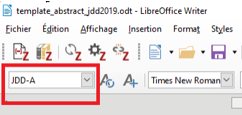
\includegraphics[width=5cm]{capture d'ecran style.png}
            \caption{\footnotesize\textbf{Capture d’écran illustrant où trouver les styles sur Libre Office }}
            \label{fig: 1 }
    \end{minipage}
    \hfill%
    \begin{minipage}[c]{.46\linewidth}
         \centering
            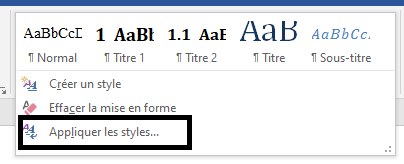
\includegraphics[width=5cm]{style sur word.png}
           \caption{\footnotesize\textbf{Capture d’écran illustrant où trouver les styles sur Word}}
            \label{fig: 2 }
    \end{minipage}
\end{figure}

    \normalsize{
    Enregistrez le fichier sous le format PDF tels que «~abstract\_nom\_prenom.pdf~».
    Par ailleurs, merci de ne pas mettre d’accent à vos noms dans le format du fichier.
    Les références étant optionnelles, vous pouvez supprimer la partie ci-dessous pour étendre votre résumé.
    }
    
\begin{flushright}
  \rule{0.85\linewidth}{3pt}
\end{flushright}

\textbf{Références (optionnelles)} {\color{red}(TNR, 11, Gras, justifié)} 

\footnotesize{$^{[1]}$ P.Nom 1, P.P. Nom 2, P.-P. Nom 3.Nom de la revue scientifique N°Vol (N°Sous Vol) (Année) Page initiale–Page finale. }

\footnotesize{$^{[2]}$ P.Nom 1, P.P. Nom 2, P.-P. Nom 3.Nom de la revue scientifique N°Vol (N°Sous Vol) (Année) Page initiale–Page finale. }

\footnotesize{$^{[3]}$ P.Nom 1, P.P. Nom 2, P.-P. Nom 3.Nom de la revue scientifique N°Vol (N°Sous Vol) (Année) Page initiale–Page finale. }

\end{document}

